%%%%%%%%%%%%%%%%%%%%%%%%% 
% Dokumentinformationen %
%%%%%%%%%%%%%%%%%%%%%%%%%
\newcommand{\titleinfo}{Cryptography and Coding Theory - Formelsammlung}
\newcommand{\authorinfo}{L.Schmid, Ch.Schlittler, S.Carriero}
\newcommand{\versioninfo}{FS2015}

%%%%%%%%%%%%%%%%%%%%%%%%%%%%%%%%%%%%%%%%%%%%%
% Standard projektübergreifender Header für
% - Makros 
% - Farben
% - Mathematische Operatoren 
%
% DORT NUR ERGÄNZEN, NICHTS LÖSCHEN
%%%%%%%%%%%%%%%%%%%%%%%%%%%%%%%%%%%%%%%%%%%%%  
% Genereller Header
\documentclass[10pt,twoside,a4paper,fleqn]{article}
\usepackage[left=1cm,right=1cm,top=1cm,bottom=1cm,includeheadfoot]{geometry}
\usepackage[english]{babel}
\usepackage[utf8]{inputenc}

% Pakete
\usepackage{amssymb}
\usepackage{amsmath}
\usepackage{bm}       % Bold Math
\usepackage{fancybox}
\usepackage{graphicx}
\usepackage{color}
\usepackage{lastpage}
\usepackage{wrapfig}
\usepackage{fancyhdr}
\usepackage{hyperref}
\usepackage{verbatim}
\usepackage{pdflscape} % landscape
\usepackage{multirow} % zellen in tabellen verbinden
\usepackage{multicol} 
\usepackage{slashbox} % getrennte zelle in tabelle
\usepackage{enumitem}
% \usepackage{array} % anordnung in tabellen

%%%%%%%%%%%%%%%%%%%%
% Generelle Makros %
%%%%%%%%%%%%%%%%%%%%
\newcommand{\formelbuch}[1]{$_{\textcolor{red}{\mbox{\small{p. #1}}}}$}
\newcommand{\verweis}[2]{ {\small (siehe auch \ref{#1}, #2 (S. \pageref{#1}))
}}
\newcommand{\subsubadd}[1]{\textcolor{black}{\mbox{#1}}}
\newenvironment{liste}[0]{
	\begin{list}{$\bullet$}{\setlength{\itemsep}{0cm}\setlength{\parsep}{0cm} \setlength{\topsep}{0cm}}}
    {\end{list}}

\newenvironment{beschreibListe}[0]{\vspace{-2mm}
	\begin{description}[noitemsep, nolistsep]\setlength{\itemsep}{0cm} \setlength{\parsep}{0cm} \setlength{\topsep}{0cm} \setlength{\parskip}{0cm}}
    {\end{description}}

    
\newcommand{\logd}[0]{\log_{10}}
\newcommand{\subsubsubsection}[1]{\textbf{#1}}

\newenvironment{aufzaehlung}[0]{
	\begin{enumerate}\setlength{\itemsep}{0cm}\setlength{\parsep}{0cm} \setlength{\topsep}{0cm} \setlength{\parskip}{0cm}} {\end{enumerate}}

\newcommand{\abbHeight}[3]{
	\begin{center}
		\includegraphics[height=#2]{./bilder/#1} \\
		#3
    \end{center}
}

\newcommand{\hilight}[1]{\colorbox{yellow}{#1}}
\newcommand{\todo}[1]{\colorbox{red}{TODO: #1}}
\newcommand{\matlab}[1]{\footnotesize{(Matlab: \texttt{#1})}\normalsize{}}
\newcommand{\tr}[2]{\large{\textit{TR: \texttt{#1}$\Rightarrow$\texttt{#2} }}\normalsize}

\newcommand{\skriptsection}[2]{\section{\texorpdfstring{#1 \formelbuch{#2}}{#1}}}
\newcommand{\skriptsubsection}[2]{\subsection{\texorpdfstring{#1 \formelbuch{#2}}{#1}}}
\newcommand{\skriptsubsubsection}[2]{\subsubsection{\texorpdfstring{#1 \formelbuch{#2}}{#1}}}
\newcommand{\skriptsubsubsubsection}[2]{\subsubsubsection{\texorpdfstring{#1 \formelbuch{#2}}{#1}}}

%%%%%%%%%%
% Farben %
%%%%%%%%%%
\definecolor{black}{rgb}{0,0,0}
\definecolor{red}{rgb}{1,0,0}
\definecolor{white}{rgb}{1,1,1}
\definecolor{grey}{rgb}{0.8,0.8,0.8}

%%%%%%%%%%%%%%%%%%%%%%%%%%%%
% Mathematische Operatoren %
%%%%%%%%%%%%%%%%%%%%%%%%%%%%
\DeclareMathOperator{\sinc}{sinc}
\DeclareMathOperator{\sgn}{sgn}



% Fouriertransformationen
\unitlength1cm
\newcommand{\FT}
{
\begin{picture}(1,0.5)
\put(0.2,0.1){\circle{0.14}}\put(0.27,0.1){\line(1,0){0.5}}\put(0.77,0.1){\circle*{0.14}}
\end{picture}
}


\newcommand{\IFT}
{
\begin{picture}(1,0.5)
\put(0.2,0.1){\circle*{0.14}}\put(0.27,0.1){\line(1,0){0.45}}\put(0.77,0.1){\circle{0.14}}
\end{picture}
}



%%%%%%%%%%%%%%%%%%%%%%%%%%%%
% Allgemeine Einstellungen %
%%%%%%%%%%%%%%%%%%%%%%%%%%%%
%pdf info
\hypersetup{pdfauthor={\authorinfo},pdftitle={\titleinfo},colorlinks=false}
\author{\authorinfo}
\title{\titleinfo}

%Kopf- und Fusszeile
\pagestyle{fancy}
\fancyhf{}
%Linien oben und unten
\renewcommand{\headrulewidth}{0.5pt} 
\renewcommand{\footrulewidth}{0.5pt} 

\fancyhead[L]{\titleinfo{ }- Summary}
%Kopfzeile rechts bzw. aussen
\fancyhead[R]{\today{ }- Page \thepage/\pageref{LastPage}}
\fancyfoot[C]{\copyright{ }\authorinfo}

% Einr�cken verhindern versuchen
\setlength{\parindent}{0pt}



% Möglichst keine Ergänzungen hier, sondern in header.tex
\begin{document} 
 
%%%%%%%%%%%%%%%%%%%%%%%%%%%%%%%%%%%%%%%%%%%%%%%%%%%%%%%%%%%%%%%%%%%%%%%%%%%%%%%%%%%%%%%%%%%%%%%
%%%%%%%%%%%%%%%%%%%%%%%%%%%%%%%%%%%%%%%%%%%%%%%%%%%%%%%%%%%%%%%%%%%%%%%%%%%%%%%%%%%%%%%%%%%%%%%

% Diskrete Fourier Transformation
%\input{files/Fourier.tex}
%\input{Content/Transformationen/Transformationen}
% Einleitung
\section{Basics}
\begin{minipage}{9cm}
\subsection{Euclidean Algorithm}
With the Euclidean Algorithm the $gcd$ is found on base of $gcd(a,b)=gcd(b,a \mod b)$ 
Pseudo code:
\begin{verbatim}
	int gcd(int a, int b){	=> a>b
		while(b \inq 0){
			r = a mod b
			a = b
			b = r
		}
		return a
	}
\end{verbatim}
The \em Extended Euclidean Algorithm \em return the $gcd(a,b)$ 
and how can it build out of $a,b$ $\Rightarrow gcd(a,b)=x a + y b$. 
e.g:\\ 
$gcd(78,99)=3=14 \cdot 78 - 11 \cdot 99$\\
\tr{eucl(a,b)}{$\{x\; y \; gcd(a,b)\}$}\negmedspace; $y=b^{-1} \mod a$\\
\tr{eucl(12,9)}{$\{1\, -\negmedspace 1 \quad 3\}$}$=12-9=3$\\
\end{minipage}
\hspace{4mm}
\begin{minipage}{9.5cm}
\subsection{Eulers Phi-Function $\varphi(n)$}
Sie gibt f\"ur jede nat\"urliche Zahl $n$ an, wie viele zu $n$ teilerfremde positve 
ganze Zahlen es gibt, die nicht gr\"osser als $n$ sind.\\
\tr{fi(n)}{$\varphi(n)$}\\ 

\begin{tabular}{| l l l |}
	\hline
	1:		&	$n=p \to p=Primzahl(PZ)$				&	$\varphi(n)=p-1$\\
	2:		&	$n=p \cdot q \to p,q=PZ$	&	$\varphi(n)=(p-1)(q-1)$\\
	3:		&	$n=p^k \to p=PZ$			&	$\varphi(n)=p^k-p^{k-1}$\\
	\hline
\end{tabular}

\subsection{Modulare Arithmetic}
$a \equiv b \mod m$ and $c \equiv d \mod m \to a=b+k \cdot m$; $k \in \mathbb{N}$ \\
\begin{liste}

\item $a \cdot c \mod m = (a \mod m) \cdot (c \mod m) \Rightarrow$ \\ Reduktion durch kleinere Zahlen
\item $a + b \mod m \equiv b \mod m + d \mod m$
\item $k a \equiv k b \mod m$
\end{liste}
\end{minipage}
\subsection{Modulares Inverses}
Definition: $a \cdot x \equiv 1 \mod m \Rightarrow x \equiv a^{-1} \mod m$\\
Tatsache: $x$ existiert genau, wenn $gcd(a,m)=1$\\
Trick: $1 = a \cdot x + m \cdot y \Rightarrow 1 \equiv a \cdot x \mod m$ (use \em Extended Euclid (a,m) \em)\\
BSP: $a = 16, b = 13; a^{-1} \mod b \equiv 5$ \\
\tr{inv(a,m)}{$a^{-1}$}

\subsection{Fermat's little Theorem}
\begin{tabular}{l l}
	$p$=prime number					&	if $\alpha$ and $p$ are coprime (coprime = Teilerfremd = $gcd(\alpha,p)=1$)\\
	$\alpha^p \equiv \alpha \mod p$		&	$\alpha^{p-1} \equiv 1 \mod p$ e.g. \\
	$a=3; p=7$ 							&   $3^6 \mod 7 \equiv 1 \mod 7$ \\\\
   $\bm{\alpha^{\varphi(m)} \equiv 1 \mod m}$  & $\Rightarrow$ if $\alpha$ and $m$ are coprime. e.g\\
   $m=15\Rightarrow\varphi(15)=\varphi(3\cdot5)=(3-1)(5-1)=8$ &  $\Rightarrow a^8\equiv 1 \mod 15$\\
\end{tabular}\\\\
Note: Fermat's little Theorem does only give an upper bond for the exponent $e$ such that $\alpha^e=1\mod p$. For some
integers $\alpha$, there may exist an exponet $e<p-1$ such as $\alpha^e \equiv 1 \mod p$.\\


\subsection{Order of Elements}
$g \in \mathbb{Z}, \quad e \in \mathbb{N}, \quad p \in \mathbb{N} \rightarrow$ kleinste Zahl $e$ sodass \boxed{g^e \equiv 1 \mod p} gibt die
Ordnung von $g \mod p$.\\
$g^n \mod m \equiv 1 $ wenn $n=k\cdot e$\\
$g^l = g^k$ wenn $l\equiv k \mod e$\\ 
$\beta = q^i \mod p \Rightarrow \beta =$ Erzeugndes modulo p wenn $gcd(p-1,i)=1$ (coprime)\\
$g$ ist Erzeugendes (generator) modulo $p$, falls die Menge der Elemente $g^i;1 \leq i \leq p-1$ gleich der Menge $\{1,\ldots,p-1\}$ ist.

\subsection{Chinese Remainder Theorem}
\begin{minipage}{8cm}
Wird verwendet um ein Gleichungssystem zu l\"osen: \\
$x \equiv a_1 \mod m_1$\\
$x \equiv a_2 \mod m_2$\\
$\ldots$\\
$x \equiv a_n \mod m_n$\\
\end{minipage}
\begin{minipage}{9cm}
$m=\displaystyle\prod_{i=1}^{n} m_i, \quad M_i=m/m_i, \quad gcd(m_i, M_i)=1, 1 \leq i \leq n$\\
$y_iM_i \equiv 1 \mod m_i \to$ \tr{eucl($m_i,M_i$)}{$\{.., y_i,.. \}$}, \\
$x=\left(\displaystyle\sum_{i=1}^{n} a_i  y_i M_i \right) \mod m=\left(\displaystyle\sum_{i=1}^{n} a_i  y_i M_i \right) \mod m_1 m_2 \ldots $
\end{minipage}\\
z.B.\\
\begin{minipage}{5cm}
$x\equiv a_1 \mod m_1 = 5  \mod 7$\\
$x\equiv a_1 \mod m_1 = 3  \mod 11$\\
$x\equiv a_1 \mod m_1 = 10 \mod 13$\\
$x=?$
\end{minipage}
\begin{minipage}{5cm}
$m=m_1 m_2 m3 = 7\cdot 11 \cdot 13 = 1001$\\
$M_1=m/m_1=11 \cdot 13 = 143$\\
$M_1=m/m_2=7 \cdot 13 = 91$\\
$M_1=m/m_3=7 \cdot 11 = 77$\\
\end{minipage}
\begin{minipage}{8cm}
Mit dem extended euclid: \\
$y_1=5;  y_2=4; y_3=12$; $M_1 y_1 \equiv 1 \mod m_1$\\
$\bm x\equiv 5\cdot5\cdot143+3\cdot4\cdot91+10\cdot12\cdot77 \equiv \bm{894} \mod 1001$\\
$\Rightarrow 894 \mod 7 \equiv 5; \quad 894 \mod 11 \equiv 3;$ etc.
\end{minipage}

\subsection{Faster Exponentiation: Square and Multiply}
Um den Modulos von grossen Potenzen zu rechnen werden die Potenzen in Zweierpotenzen heruntergebrochen und Schritt für Schritt ausgerechnet:\\
$g^e=g^{\sum c_i 2^i}=\prod_{i=0}^k \left(g^{2^i}\right)^{e_i}$
\begin{aufzaehlung}
\item Drücke die gegebene Potenz in Zweierpotenzen aus: $e=73=2^0+2^3+2^6$
\item Berechne die Zweierpotenzen $g^{2^i} \mod m$ und reduziere nach jeder Berechnung: $g=6\Rightarrow$\\ 
$6^{2^1} \mod 100 = 36;\quad 6^{2^2} \mod 100 \equiv 36^2  \mod 100 \equiv -4;\quad  6^{2^3} \mod 100 \equiv {-4}^2 \mod 100 \equiv 16; \ldots$
\item Berechne das Produkt der Zweierpotenzen: $6^{2^0}\cdot6^{2^3}\cdot6^{2^6}\mod 100\equiv 36 \cdot 16 \cdot -4 \equiv 16$
\end{aufzaehlung}
Mit Hilfe des \em Square and Multiply \em wird der Rechenaufwand auf $\log_2(e)$ Potenzen und auf $1/2 \log_2(e)$ Multiplikationen reduziert.

\subsection{Glossar}
\begin{minipage}{12.5cm}
\begin{tabular}[]{|l |p{9cm}| }
	\hline
	bijektiv			&	umkehrbar eindeutig		\\
	\hline
	injektiv			&	Sie besagt, dass jedes Element der Zielmenge $Y$ einaml als Funktionswert angenommen wird.
							Es werden also keine zwei verschiedenen Elemente der Definitionsmenge $X$ auf dasselbe Element in 
							der Zielmenge $Y$ abgebildet.		\\
	\hline
	permutation			&	(Vertauschen) versteht man die Ver\"anderung der Anordnung von Objekten in einer Reihenfolge
							durch Vertauschen der Elemente.			\\
	\hline
	affine Abbildung	&	lineare Abbildung, es bleibt Kolinearit\"at, Parallelit\"at und Teilerverh\"altnisse erhalten.	 \\
	
	\hline
\end{tabular}\\

\end{minipage}
\begin{minipage}{6cm}
\textbf{Irreduzible Polynome in:}\\
\begin{tabular}{l l}
	$GF(2)$				&	$GF(3)$\\
	\hline
	$x$					&	$x^2+1$\\
	$x+1$				&	$x^2+x-1$\\
	$x^2+x+1$			&	$x^2-x-1$\\
	$x^3+x+1$			&	$x^3-x+1$\\
	$x^3+x^2+1$			&	$x^3-x-1$\\
	$x^4+x+1$			&	$x^3+x^2+x-1$\\
	$x^4+x^3+1$			&	$x^3+x^2-x+1$\\
	$x^4+x^3+x^2+x+1$	&	$x^3+x^2-1$\\ 
						&	$x^3-x^2+1$\\ 
						&	$x^3-x^2+x+1$\\ 
						&	$x^3-x^2-x-1$\\ 
\end{tabular}
\end{minipage}







\section{Asymmetric (Public Key) Cryptography}
\label{sec::CrypCod_Asymmetric Crypto}
\begin{tabular}{|l| p{14.7cm}|}
	\hline
	Diffie-Hellmann				 	& 	Choose a large public prime $p$ and a generator $a \in GF(p)$.\\
	Key Exchange					&	1. $A$ chooses a large random integer $x$, computes $a^x \mod p = c_1$ and sends the result to $B$. \\
									&	2. $B$ chooses a large random integer $y$, computes $a^y \mod p = c_2$ and sends the result to $A$. \\
									&	3. $A$ and $B$ compute each the secret key: $A: c_2^x \mod p=k $ and $B: c_1^y \mod p=k \to k=a^{xy} \mod p$.\\
									& 	The security is base on the assumption that the discrete logarithm $x=\log_{a}(c_1)$ hard to compute is.\\
									&	This assumption will be definitely wrong for quantum computer!!!\\
	\hline
	RSA public key 					&	$p$ and $q$ are primes \\
	cryptosystem key				&	$n=pq$ and $ed\equiv 1 \mod \varphi(n) \Rightarrow e d = \varphi(n) \cdot i + 1$\\
	generation:						&	public key: $(n,e)$, secret key: $(n,d), p,q, \varphi(n)$\\
									\cline{2-2}
									&	1. $A$ looks up the pulbic key $(n,e)$ of $B$\\
	encryption/decryption:			&	2. $A$ encrypt message $m \to c$: $c \equiv m^e \mod n$.\\
									&	3. $A$ sends the ciphertext $c$ to $B$.\\
									&	4. $B$ decrypts $c$ by computing $m\equiv c^d \mod n \equiv (m^{e})^d \equiv  m^{\varphi(n) \cdot i + 1} \equiv  \left(m^{\varphi(n)}\right)^i \cdot m \mod n$\\
									&	$\xrightarrow[m^{\varphi(n)} \mod n\equiv 1]{\text{little Fermat}} m \mod n \equiv m $\\
									\cline{2-2}
	signature						&	$s=m^d \mod n$ only owner of $(n,d)$ can compute this.\\
									&	$m=s^e \mod n$ every with public $(n,e)$ can compute this.\\
									&	$\Rightarrow$ often only the hash $h(m)$ is signated. Attention: 
										collisions $h(m_1)=h(m_2)$.\\
	\hline
\end{tabular}
\section{Symmetric Cryptography}
Block Ciphers: map blocks of symbols of fixed length $n$ into blocks of the same length.\\
\begin{tabular}{|l l |l|}
	\hline
	Vigenère Cipher &	encryption	&	$E_z: \mathbb{Z}_m^n \to \mathbb{Z}_m^n, \mathbf{v} \mapsto \mathbf{v} + \mathbf{z} \mod m$ \\
							         \cline{2-3}
	(16th century) & decryption & $D_z: \mathbb{Z}_m^n \to \mathbb{Z}_m^n, \mathbf{v} \mapsto \mathbf{v} - \mathbf{z} \mod m$ \\
	\hline
	Hill Cipher & encryption & $E_M: \mathbb{Z}_m^n \to \mathbb{Z}_m^n, \mathbf{v} \mapsto M\mathbf{v} \mod m$ \\
							         \cline{2-3}
	(1929) & decryption & $D_M: \mathbb{Z}_m^n \to \mathbb{Z}_m^n, \mathbf{v} \mapsto M^{-1}\mathbf{v} \mod m$ \\
	& & $M$ is an $(n \times n)$-matrix with elements in $\mathbb{Z}_m$ \\
	\hline
	General & encryption & $E_{(M,\mathbf{b})}: \mathbb{Z}_m^n \to \mathbb{Z}_m^n, \mathbf{v} \mapsto M\mathbf{v} + \mathbf{b} \mod m$ \\
							         \cline{2-3}
	affine linear cipher & decryption & $D_{(M,\mathbf{b})}: \mathbb{Z}_m^n \to \mathbb{Z}_m^n, \mathbf{v} \mapsto M^{-1}\mathbf{v} - \mathbf{b} \mod m$ \\
	\hline
\end{tabular}

\subsubsection{Cryptanalysis of historical block ciphers}
\begin{tabular}{|cccccccccccccccccccccccccc|} %{llllllllllllllllllllllllll}
	\hline
	a & b & c & d & e & f & g & h & i & j & k  & l  & m  & n  & o  & p  & q  & r  & s  & t  & u  & v  & w  & x  & y  & z  \\
	0 & 1 & 2 & 3 & 4 & 5 & 6 & 7 & 8 & 9 & 10 & 11 & 12 & 13 & 14 & 15 & 16 & 17 & 18 & 19 & 20 & 21 & 22 & 23 & 24 & 25 \\
	\hline
\end{tabular}\\
Modulus $m=26$\\

Need: $n+1$ plaintexts $\bm w_i$ and the corresponding ciphertexts $\mathbf{c}_i= M\mathbf{w}_i+ \mathbf{b} \mod m$.\\
$W=(\bm w_1-\bm w_0, \ldots , \bm w_n-\bm w_0)  \mod m$ and $C=(\bm c_1-\bm c_0, \ldots , \bm c_n-\bm c_0) \mod m$ \\
$\Rightarrow \text{if } gcd(det(W),m)=1 \text{ then } M=CW^{-1} \mod m$ and $\bm b=\bm c_0-M\bm w_0 \mod m$.\\
For Hill cipher we set $\bm w_0=\bm c_0 = \bm 0 \Rightarrow \bm b=0$; For Vigen\'{e}re cipher we set the $M = I$\\
Without knowledge of the plaintext, the plaintext can be estimated with the known statistics of a language. 

\subsubsection{Secure Block Ciphers}
The plaintexts $X$ and ciphertexts $Y$ are bit strings of length $n$ and the keys $K$ are bit strings of length $r$. Then a cryptographic algorithm $E$ defines equations that hold for each ciphertext bit:\\
\begin{minipage}{0.25\linewidth}
$y_1 = F_1(x_1,\ldots,x_n,k_1,\ldots,k_r)$\\
$\ldots = \ldots$\\
$y_n = F_n(x_1,\ldots,x_n,k_1,\ldots,k_r)$
\end{minipage}
\begin{minipage}{0.35\linewidth}
\textbf{Confusion:}
\begin{liste}
	\item $F_i$ should be mathematically complex
	\item For a given $\mathbf{x}$ and $\mathbf{y}$, it is not feasible to solve for $\mathbf{k}$
	\item $F_i$ must not be linear
\end{liste}
\end{minipage}
\begin{minipage}{0.35\linewidth}
\textbf{Diffusion:}
\begin{liste}
	\item Changing a single bit in the plaintext (or the key), on average $50\%$ of the ciphertext bits should change
	\item ''Every ciphertext bit should depend on every plaintext and every key bit''
\end{liste}
\end{minipage}

To achieve confusion and diffusion, many block ciphers are product ciphers: $E = E_R \circ E_{R-1} \circ \ldots \circ E_2 \circ E_1$ where $E_i$ are round functions and each uses a round key that is derived from the secret key (key scheduling) and $R$ is the number of rounds.
Nonlinearity is achieved using S-boxes: $S: \mathbb{Z}_2^m \rightarrow \mathbb{Z}_2^n$.
Security is achieved by sufficiently many rounds!

\subsubsection{Modes of Operation of Block Ciphers}%TODO: continue
Notation: $IV$ = Initial Vector, $P_i$ = Plaintext, $C_i$ = Cipher, $E_k(x)$ = encryption function with key $k$, $D_k(x)$ = decryption function with key $k$\\
\begin{tabular}{|l l |p{12cm}|}
\hline
	ECB	&	Electronic Code Book Mode	&	plaintext divided into $n$-bit blocks. Each block encryped by $E$ individually. \\
		&								&	Drawback: same plaintext goes into same cipher $\to$ gives information about the plaintext or the order of the ciphertext can be changed.\\
\hline
	CBC	&	Cipher Block Chaining Mode	&	enc: $C_1=E_k(P_1 \oplus IV), \quad C_i=E_k(P_i \oplus C_{i-1})$ \\
		&								&	dec: $P_1=D_k(C_1) \oplus IV, \quad P_i=D_k(C_i) \oplus C_{i-1}$	\\	
\hline
	CFB &	Cipher Feedback Mode		& 	enc: $C_1=P_1 \oplus E_k(IV), \quad C_i=P_i \oplus E_k(C_{i-1})$\\
		&								&	dec: $P_1=C_1 \oplus E_k(IV), \quad P_i=C_i \oplus E_k(C_{i-1})$\\
		&								&	Drawback: error propagation. Benefit: selfsync.\\
\hline
	OFB	&	Output Feedback Mode		& 	enc: $C_1=\underbrace{E_k(IV)}_{\tilde{C_1}} \oplus P_1, \quad C_i=\underbrace{E_k(\tilde{C}_{i-1})}_{\tilde{C_i}} \oplus P_i $\\
		&								& 	dec: $P_1=E_k(IV) \oplus C_1, \quad P_i=E_k(C_{i-1}) \oplus C_i $\\
		&								&	Drawback: not self synchronizing. Each message needs a different IV.\\
\hline
	CTR	&	Counter Mode				& 	enc: $C_i=P_i \oplus E_k(ctr_i) $, $ctr_i$: counter reading.\\
		&								&	dec: $P_i=C_i \oplus E_k(ctr_i) $\\
		&               & Drawback: each counter value only once $\rightarrow$ Nonce. Benefit: enc/dec parallel, no error propagation.\\
\hline
\end{tabular}\\

Period: $\approx 2^{\frac{n}{2}} \to $ birthday paradox. After about $2^{\frac{n}{2}}$ encryptions, the output of the block cipher repeats.

\subsection{DES (Data Encryption Standard)}
\begin{minipage}{10cm}
\begin{liste}
\item 16 Rounds with 56bit (thank you NSA) key each. 64bits of plaintext are ciphered. Nonlinearity comes from S-Boxes.
\item IP $=$ Initial Permutation, FP $=$ Final Permutation
\item One Round looks like: $T(L,R)=(L \oplus F_k(R),R)$ and $M(L,R)=(R,L)$
\item Transformations are involutions $\to$ two times the same operation gives the initial value.
\item $C=IP^{-1} \circ T_{16} \circ M \circ T_{15} \circ \ldots \circ M \circ T_1 \circ IP(P)$
\item $P=IP^{-1} \circ T_1 \circ  M \circ T_2 \circ \ldots \circ M \circ T_{16} \circ IP(C)$
\end{liste}
The $F$-Function works as follows:
\begin{liste}
\item The input (32-bit) is extended to 48-bit with some bits copied. Additionally the bits are permuted. ($E$-Box)
\item The data is now XOR-added with the 48-bit round key and put into 8 S-boxes.
\item The S-boxes have a nonlinear function and map the 8 different 6-bit input to 4-bit. ($S$-Boxes)
\item The output bits are permuted again. ($P$-Boxes)
\end{liste}
The big disadvantage is, that the DES algorithm just uses a 56bit key.\\
To avoid this disadvantage the Double DES was developed with the drawback of meet-in-the-middle attack. It works like this:
\begin{aufzaehlung}
    \item For every possible $DES$ key $k_i$, compute $M_i = DES(C,k_i)$ and store the tuple $(M_i, k_i)$.\\
    \item Loop again through all possible $DES$ keys $k_j$ and compute $N_j = DES^{-1}(C,k-j)$. Check whether $N_j$ 
    is the same as one of your stored $M_i$. If you find a match, it's pretty likely that you've just 
    found the two keys you're looking for!\\
    (1. table with $2^{56}$ 64bit keys, 2. table with $2^{56}$ 64bit keys $\to$ $2^{112-64} = 2^{48}$ analogies.)\\
\end{aufzaehlung}
Notes:
\begin{liste}
	\item DES is very efficient to implement in hardware, but not so in software.
  \item Better solution: Triple DES $\to$ key size = 112-bit or 168-bit.
  \item Better solution: IDEA is very efficient to implement in software, but not so in hardware (128-bit key and multiplications instead of S-Box).
\end{liste}


\subsection{AES (Advanced Encryption Standard)}
Some marketing numbers: 128 bit block size, 128, 192 or 256 bit keys. AES is an iterated block cipher with n number of $N_r$ rounds
with $N_{r_{128}}=10, N_{r_{192}}=12, N_{r_{256}}=14$. Drawback: encryption differs from decryption.\\
One round of AES consist of three layers:\\
- Nonlinear Layer: 16 parallel 8$\times$8-bit S-boxes with optimal nonlinearity.\\
- Linear Mixing Layer: Effects good diffusion.\\
- Key Additon Layer: Usual XOR of the round key with the actual internal state.\\

\end{minipage}
\hspace{5mm}
\begin{minipage}{7cm}
\begin{center}
  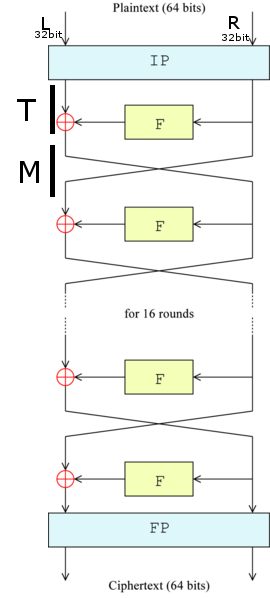
\includegraphics[width=5.5cm]{./bilder/DES-main-network.png}\\
  Schemata of the \em DES main network \em\\
  \vspace{2mm}
  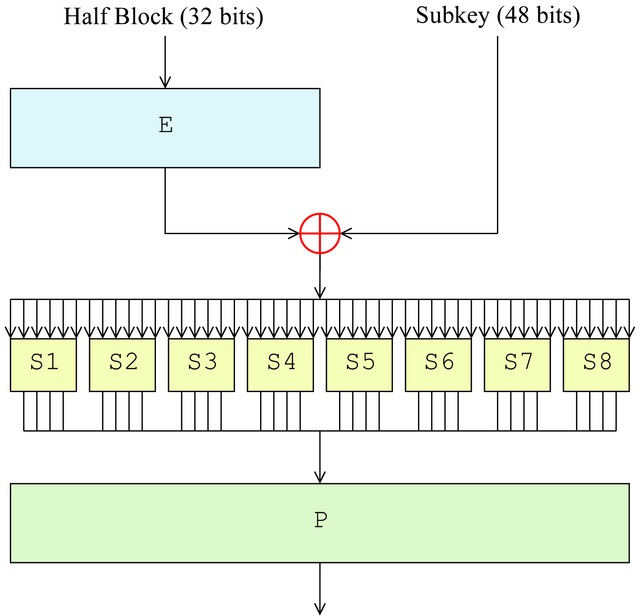
\includegraphics[width=7cm]{./bilder/DES-f-function.png}\\
  Schemata of the DES \em F\em-Function\\
 \end{center}
\end{minipage}

\begin{multicols}{2}
Encryption-pseudocode:
\begin{verbatim}
Store input bits into state matrix
AddRoundKey
while (Count rounds from 1 to NumberOfRounds-1) {
  SubBytes
  ShiftRows
  MixColumns
  AddRoundKey
}
SubBytes
ShiftRows
AddRoundKey
Return state matrix
\end{verbatim}

\textbf{AddRoundKey:}
XOR each column of the state matrix with the corresponding word from the round key.

\textbf{SubBytes:}
Take the multiplicative inverse in GF($2^8$) (map $\{00\}$ to $\{00\}$), then: affine Transformation over GF($2^8$).

\textbf{ShiftRows:}
Bytes in the last three rows of the state are cyclically shifted over different number of byte.

\textbf{MixColumns:}
Columns are considered as polynomials over GF($2^8$) and multiplied modulo $x^4+1$ with a fixed polynomial: $a(x) = \{03\} \cdot x^3 + \{01\} \cdot x^2 + \{01\} \cdot x + \{02\}$
\end{multicols}

\subsection{IDEA (International Data Encryption Algorithm)}
\begin{multicols}{2}
\begin{liste}
	\item 128-bit key
	\item Confusion: Mixes three ''incompatible'' group operations so that no two successive operations are of the same type.
	\item Diffusion: Provided for by the ''Multiply-Add (M-A) Box''.
	\item Encryption/Decryption similarity: Differ only in the key schedule used.
	\item Scalable: Mini-versions (2,4,8-bit symbols) can be used for analysis.
	\item Transparency: No ''random-looking'' tables or ''mysterious'' S-boxes.
	\item Easy to substitute for DES: Both have 64-bit plain-/ciphertexts
\end{liste}

Operations:
\begin{liste}
	\item [\-] $\oplus$ Bit-by-bit modulo-two addition (XOR)
	\item [\-] $\boxplus$ Addition modulo $2^{16}$
	\item [\-] $\odot$ Multiplication modulo $2^{16} + 1$ of nonzero numbers
\end{liste}
The output of one operation never goes to another operation of the same kind $\rightarrow$ Confusion.

\begin{minipage}{0.5\linewidth}
Multiply-Add Box:\\
Provides Diffusion. This is the simplest structure with this property!
\end{minipage}
\begin{minipage}{0.5\linewidth}
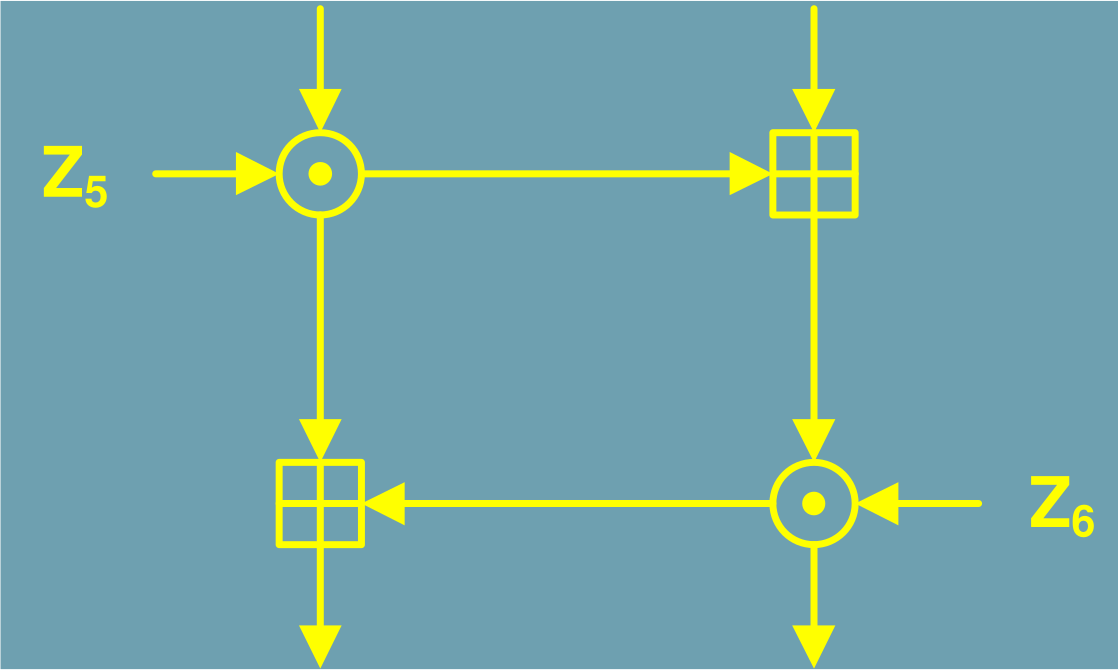
\includegraphics[width=0.8\linewidth]{./bilder/MultiplyAdd.png}
\end{minipage}

\vfill\null
\columnbreak
\begin{minipage}{\linewidth}
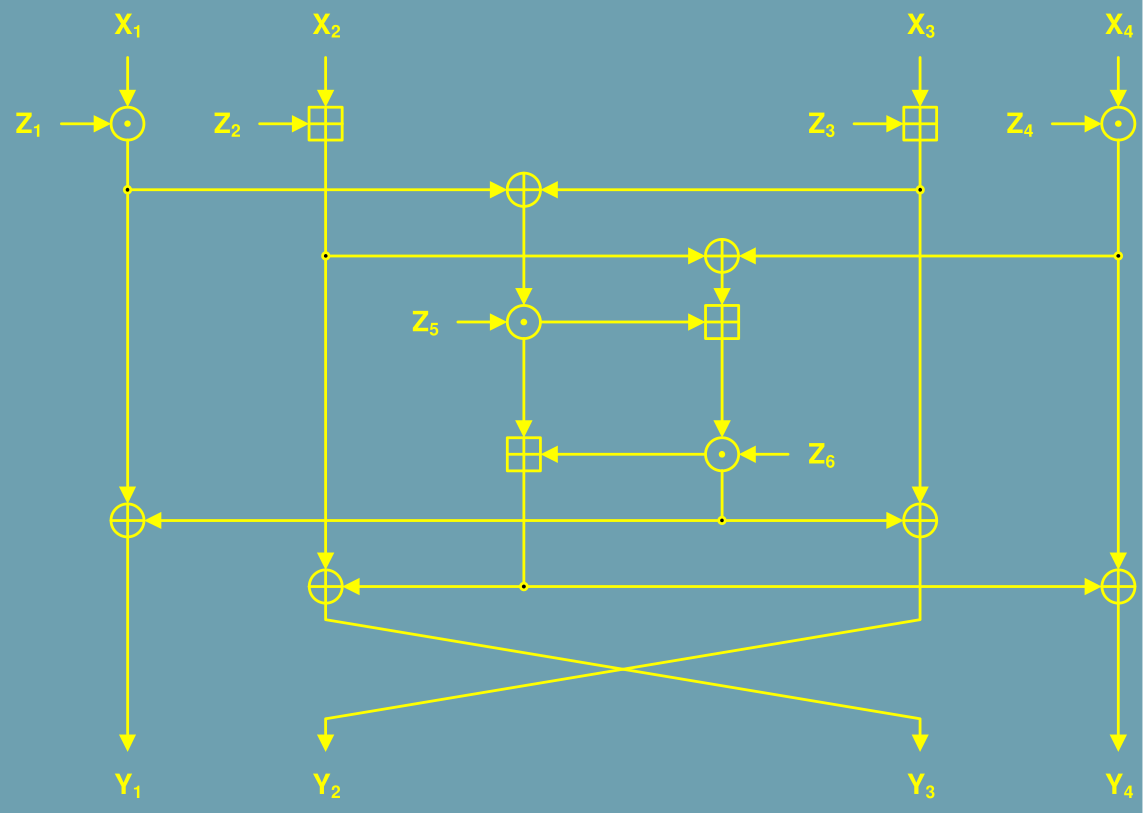
\includegraphics[width=0.8\linewidth]{./bilder/IDEA_structure.png}\\
An IDEA encryption round, $Z_1, \ldots, Z_6$: Round keys (16 bits)\\
\end{minipage}

Final round:\\
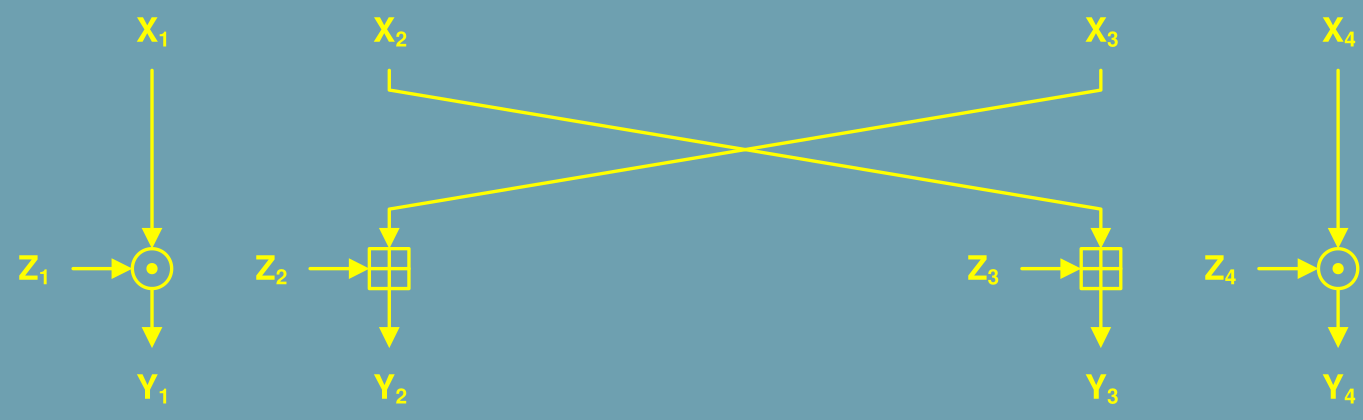
\includegraphics[width=\linewidth]{./bilder/IDEA_final_round.png}
Causes that the same structure can be used to encrypt and decrypt (just use the inverses of the round keys in reverse order).
\end{multicols}

\subsection{PGP (Pretty Good Privacy)}
PGP uses block ciphers and is used for file encryption on a computer, computation of private and public RSA keys, and for sending and receiving of encrypted emails.\\
PGP is a set of different methods.\\
Necessary steps:
\begin{aufzaehlung}
\item A session key is generated.
\item The message is encrypted with a block cipher unsing the session key (IDEA and other block ciphers).
\item RSA is used to encrypt the session key with the public key of the receiver.
\item The encrypted message and the encrypted session key are bundled to a message that is mailed to the receiver.\\
\end{aufzaehlung}
PGP works without public key infrastructure (web of trust is used).

\subsubsection{Conclusion}
\begin{liste}
\item AES fast, RSA (based on Diffie-Hellmann) slow
\item AES need previous knowledge 
\item RSA for key-exchange, and AES/IDEA/DES for message cipher.
\end{liste}

% Einleitung
\section{Elliptic Curve}
Elliptic curve equation: $y^2=x^3+a\cdot x+b \quad a,b,x,y \in \mathbb{R}$  $\to $
If an elliptic curve contains multiple roots, it cannot be used to form a group ($\to 4 \cdot a^3 + 27 \cdot b^2 \neq 0$).\\
The negative of a point $P \equiv (x_p, y_p)$ is its reflection on the x-axis $\to$ $-P \equiv (x_p, -y_p)$.
Both points lie on the curve.\\
Note: When in $\mathbb{F}_p$, all calculations are done with $\mod p$.
The point at infinity $\mathcal{O}$ is the additive identity of the elliptic curve group.

\subsection{Addition}
\begin{minipage}{12.5cm}
Add two Points $P,Q$ on an Elliptic Curve. This is possible, if $4a^3+27b^2\neq0$
(Group patterns possible).\\
Geometric:\\
1. line through $P,Q \to$ intersection point $(-R)$.\\
2. Mirror on x-axis $\to R$.\\
Formula: $P+Q=R$\\

$m=\begin{cases}
\frac{3 \cdot x_p^2 + a}{2 \cdot y_P} & $ If $ P = Q\\
\frac{y_P-y_Q}{x_P-x_Q}               & $ If $ P \neq Q, P \neq -Q\\
\end{cases}$


$x_R = m^2 -x_p -x_Q$ \\
$y_R = m(x_P-x_R)-y_p$\\
$\mathcal{O}+\mathcal{O}=\mathcal{O}, \quad P + \mathcal{O} = \mathcal{O} + P = P, \quad P+ (-P) = \mathcal{O}, \quad \mathcal{O}$: point at infinity.\\

\end{minipage}
\begin{minipage}{5.5cm}
  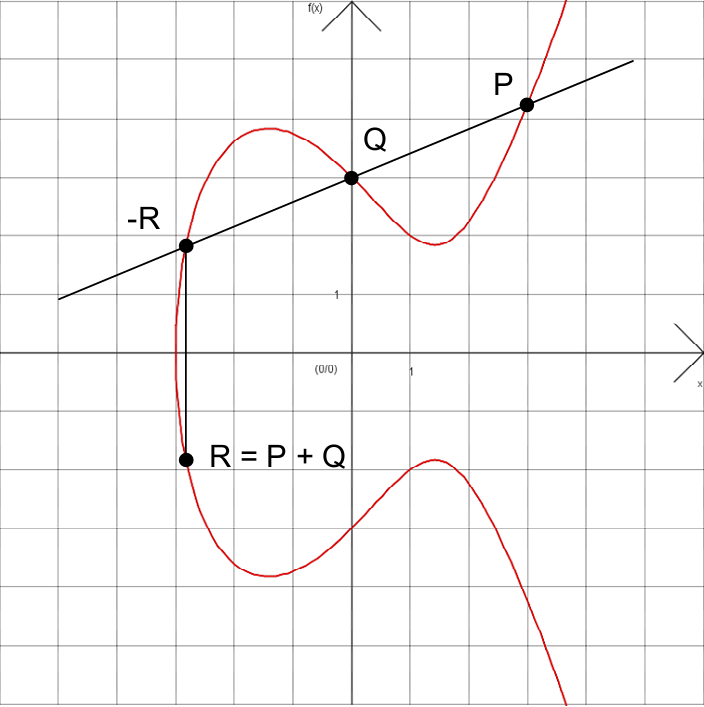
\includegraphics[width=5.5cm]{./bilder/elipticCurve.png}\\
\end{minipage} \\

\begin{minipage}{12.5cm}
\subsection{Doubling P}
Geometric:\\
1. tangent line to curve at point $P \to -R$\\
2. Mirror on x-axis $\to R$\\
Formula: $P+P=2P=R$
\end{minipage}
\begin{minipage}{5.5cm}
	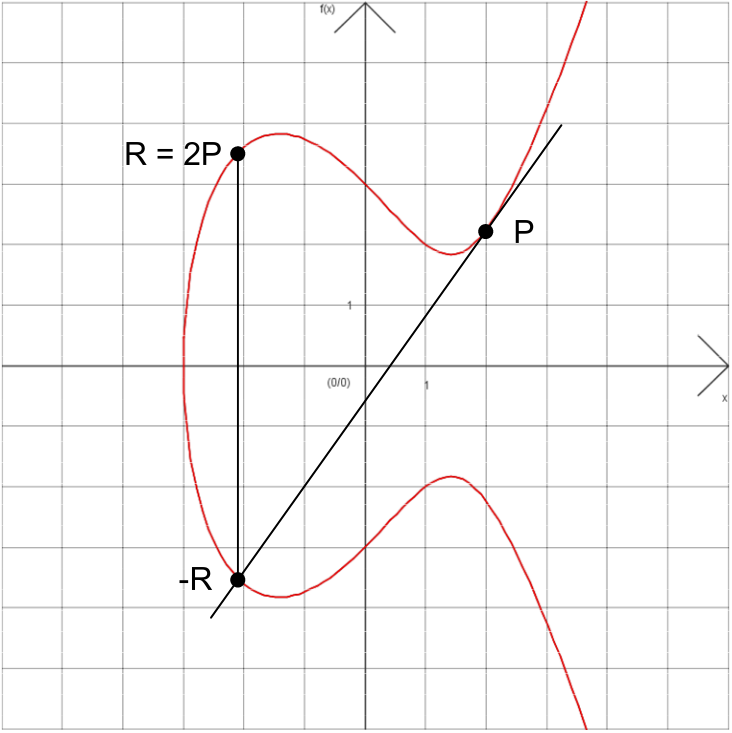
\includegraphics[width=5.5cm]{./bilder/ellipticCurveDoubling.png}
\end{minipage}

\subsection{Number of Points and Order of a Point}
In cryptology elliptic curves with a high number of points are preferred.
Number of points on the elliptic curve $E(\mathbb{F}_p)$: $\#E(\mathbb{F}_p)=p+1-t$ with $|t| \leq 2 \cdot \sqrt{p}$ \\
For large $p$:  $\#E(\mathbb{F}_p) \approx p $ \\
For small $p$:  Calculate all the possible points of the curve and add $\mathcal{O}$.\\
\begin{minipage}{8cm}
	Example: $E: y^2=x^3-1$ over $\mathbb{F}_5$\\
	\begin{tabular}{|l |l|}
		\hline
		Possible values for $y$	&	Possible values for $x$\\
		\hline
		$0^2 \mod 5 = 0$		&	$0^3 - 1 \mod 5 = 4$\\
		\hline
		$1^2 \mod 5 = 1$		&	$1^3 - 1 \mod 5 = 0$\\
		\hline
		$2^2 \mod 5 = 4$		&	$2^3 - 1 \mod 5 = 2$\\
		\hline
		$3^2 \mod 5 = 4$		&	$3^3 - 1 \mod 5 = 1$\\
		\hline
		$4^2 \mod 5 = 1$		&	$4^3 - 1 \mod 5 = 3$\\
		\hline
	\end{tabular}
\end{minipage}
\begin{minipage}{10cm}
	As for the X-Values we got some results corresponding on the Y-side, we can combine them to evaluate the points of the curve: (0/2, (0/3), (1/0), (3/1), (3/4), $\mathcal{O}$.
	So, in total the given curve has 6 points.\\
\end{minipage}\\

The order of a point $P$ can be found by point multiplication: $n \cdot P=P+P+...+P$ for $n$ times $\to n$ is the smallest non-negative integer for which $n \cdot P=\mathcal{O}$.
The order of a point always divides the total number of points. 
When calculating a new point, if $m\to \infty$ then the new point is at infinity, i.e. $\mathcal{O}$.\\

\subsection{Elliptic Curve Domain Parameters}
\begin{tabular}{l l p{11cm}}
	$T=(p,a,b,G,n,h)$	&	$p$		&	a prime $p$ specifying the finite field $\mathbb{F}_p$ \\
						&	$a,b$	&	two elements $a,b \in \mathbb{F}_p$ specifying an elliptic curve $E(\mathbb{F}_p)$ by the equation
										$E: y^2=x^3+ax+b \mod p$ \\
						&	$G$		&	a base point $G \equiv (x_g, y_g)$ on $E(\mathbb{F}_p)$\\
						&	$n$		&	$n$ which is the order of $G \to$ the smallest non-negative number $n$, for which $nG=\mathcal{O}$.\\
						&	$h$		& 	$h$ is an integer which is the cofactor; order of Point always divides the total number of points: $h=\frac{ \#E(\mathbb{F}_p) }{n}$ \\
\end{tabular}\\

For cryptographic applications the order $n$ of $G$ must be a large prime with $\lceil \log_2(n) \rceil \geq 160$ (bit) and the cofactor $h$
should be a small number with $\lceil \log_2(h) \rceil \leq 10$ (bit).

\subsection{ECDH (Elliptic curve Diffie-Hellman)}

\begin{tabular}{l p{15cm}}
	1.	&	Alice and Bob agree upon a set of elliptic curve domain parameters $T=(p,a,b,G,n,h)$. \\
	2.	&	Alice randomly chooses a secret integer $d_A$ in the interval $[1,n-1]$ and computes $Q_A=d_A \cdot G$.\\
	3.	&	Bob randomly chooses a secret integer $d_B$ in the interval $[1,n-1]$ and computes $Q_B=d_B \cdot G$.\\
	4.	&	Alice and Bob exchange $Q_A$ and $Q_B$. The integers $d_A$ and $d_B$ are kept secret.\\
	5.	&	Alice computes $P_A=d_A \cdot Q_B$. Afterwards, $d_A$ can be deleted. \\
	6.	&	Bob computes $P_B=d_B \cdot Q_A$. Afterwards, $d_B$ can be deleted. \\
		&	\\
		&	The points $P_A$ and $P_B$ are equal, since $P_A=d_A \cdot Q_B = d_A \cdot d_B \cdot G = d_B \cdot Q_A = P_B \to P_A = P_B = P$.\\
		&	\\
	7.	&	If $P \neq \mathcal{O}$ then Alice and Bob take the x-coordinate $x_p$ as the shared key.
\end{tabular}

Note that the secret keys $d_a$ and $d_b$ are never transmitted over the unsecure channel.
However, the eavesdropper knows $G$ and $d_a \cdot G$ (and $d_b \cdot G$).
Thus, the scheme is only secure if it is practically impossible to compute $d_a$ (or $d_b$) from $G$ and $d_a \cdot G$ (or $d_b \cdot G$).
This problem is known as the ECDLP.

\subsection{ECDLP (Elliptic Curve Discrete Logarithm Problem)}

Given an elliptic curve $E(\mathbb{F}_p)$ over a finite field $\mathbb{F}_p$, a point $G$ on that curve and another point $Q$ you know to be an integer multiple of $G$.
The problem is to find the integer $n$ such that $nG=Q$.\\
The security of elliptic curve cryptography rests on the assumption that the elliptic curve discrete logarithm problem is hard to solve.

\subsection{ECDSA (Elliptic Curve Digital Signature Algorithm)}
We start with an elliptic curve $E(\mathbb{F}_p)$ over a finite field $\mathbb{F}_p$ and a base point $G$ of order $n$.\\
To sign the message m, Alice generates a key pair $d_A, Q_A$, where $d_A$ is an integer randomly chosen in the interval $[1,n-1]$.
She computes the public key $Q_A = d_A \cdot G$.
Then, Alice does the following:\\
\begin{tabular}{l l}
	1. 	&	Select a random integer $k$ with $1 \leq k \leq n-1$. \\
	2. 	&	Compute $k \cdot G \equiv (x_1, y_1)$. \\
	3. 	&	Compute $r = x_1 \mod n$. If $r = 0$ then go to step 1.\\
	4. 	&	Compute $k^{-1} \mod n$.\\
	5. 	&	Compute $e = Hash(m)$.\\
	6. 	&	Compute $s=k^{-1} \cdot (e+d_A \cdot r) \mod n$. If $s = 0$ then go to step 1.\\
	7. 	&	Alice'x signature for the message $m$ is $(r, s)$.\\
\end{tabular}\\

To verify Alice's signature $(r, s)$, Bob must obtain an authentic copy of Alice domain parameters
and public key $Q_A$. Bob then does the following:\\
\begin{tabular}{l l}
	1. 	&	Verify that $r$ and $s$ are integers in the interval $[1, n-1]$.\\
	2. 	&	Compute $e = Hash(m)$.\\
	3. 	&	Compute $w = s^{-1} \mod n$.\\
	4. 	&	Compute $u_1 = e \cdot w \mod n$ and $u_2 = r \cdot w \mod n$.\\
	5. 	&	Compute $X = u_1 \cdot G + u_2 \cdot Q_A \equiv (x_1, y_1)$.\\
	6. 	&	If $X = \mathcal{O}$ then reject the signature. Otherwise compute $v = x_1 \mod n$.\\
	7. 	&	Accept the signature if and only if $v = r$.\\
\end{tabular}


% Einleitung
\section{Digital Signature}
Fundamentals:
\begin{liste}
  \item	\textbf{Authentication}: Who sent the message. It's really him?
  \item \textbf{Integrity}: Is the message still the same what the sender sent.
  \item \textbf{None-repudiation}: an entity cannot deny having signed it.
\end{liste}


\subsection{RSA  Signature}
The RSA signature is build as in chapter \ref{sec::CrypCod_Asymmetric Crypto} - \nameref{sec::CrypCod_Asymmetric Crypto} on page 
\pageref{sec::CrypCod_Asymmetric Crypto}.
\subsubsection{Attacks to RSA Signature}
\subsubsubsection{Man in the Middle/ Authentication of public key}: 
Is one of the most common and dangerous attacks. The base of this attacks is that the attacker is sending you his public key and 
tell you it's the original key. Then he forward all the traffic (key exchange data) from him to the original page. 
He can now listen to all the crypted traffic.\\
\subsubsubsection{No message attack}: For this the attacker generate a arbitrary number $s$ an compute the the message $m=s^e\mod n$
The message $m$ has yet no structure, no useful content, but it's signed by Alice. To avoid this, the message should have some redundancy as hash value,
checksum, etc.\\
\subsubsubsection{Common modulus attack}: $c_e=m^f \mod n \quad c_f=m^f \mod n$, known: $c_e,c_f,(n,f),(n,e)$ then $1=x \cdot e + y \cdot f$
$\rightarrow (c_e)^x \cdot (c_f)^y=(m^e)^x \cdot (m^f)^y=m^{ex+yf} \equiv m^1 \mod n$.

\subsubsubsection{Multiplicative Property of RSA}: 
\begin{aufzaehlung}
\item The attacker would like Alice to sign message m without showing the true content to her.
\item He chooses any $m_1$ with $gcd(m_1,n)=1$
\item He computes $m_2 = m \cdot m_1^{-1} \mod n$
\item He asks Alice to sign $m_1 \& m_2$ and receives $s_1 \& s_2$
\item $s=s_1 \cdot s_2 \mod n \equiv (m_1\cdot m_2)^d \mod n \equiv m^d \mod n$ is the valid signature of m
\end{aufzaehlung}
Some redundancy in the messages can avoid this attacks. Also Alice should sign some ``random'' messages.

\subsection{DSA Digital Signature Algorithm}

Generate a public key $(\bm {p,q,g,y})$ and the secret key $x:$
\begin{aufzaehlung}
\item select a prime number $\bm q$ with exact 160 binary digits $(2^{159}< \bm q < 2^{160})$
\item select a prime number $\bm p$ between 512 and 1024 binary digits $(2^{511+64t}< \bm p < 2^{512+64t})$
\item select a number $1< h<\bm p$ and compute $\bm g = h^{\frac{p-1}{q}} \mod p$ if g=1 repeat this step.
(compute a generator of subgroup of order $q \mod p$)
\item select a random integer $1 \leq \bm x \leq \bm q-1$
\item compute $\bm y=\bm g^{\bm x} \mod \bm p$
\end{aufzaehlung}
Sign a hash $h(m):$ and return signature $(\bm {r,s})$
\begin{aufzaehlung}
\item Select a random integer $0< k<q$
\item $\bm r = (\bm g^k \mod \bm p) \mod \bm q$
\item $s=(k^{-1} \cdot (h(m) + \bm x\cdot \bm r))\mod \bm q$
\end{aufzaehlung}
Verification with public key $(\bm {p,q,g,y})$ and signature $(\bm {r,s})$:
\begin{aufzaehlung}
\item check if $\bm r \& \bm s$ is in range $<\bm q$
\item $w=(s^{-1})\mod\bm q$
\item $u_1=( w\cdot h(m)) \mod \bm q$
\item $u_2=( w \cdot \bm r) \mod\bm q$
\item $\bm v=((\bm g^{u_1}\bm y^{u_2})\mod \bm  p) \mod \bm q$
\item if $\bm v= \bm r \Rightarrow$ Accept it!
\end{aufzaehlung}



\subsection{ElGamal}
Find primitive roots in a given field $\mathbb{F}_p$.
\begin{aufzaehlung}
\item Factor $p-1=p_1^{e1} \cdot p_2^{e2} \ldots p_k^{ek}$
\item Choose a random element $\alpha$ in $\mathbb{F}_p$ with $2 \leq \alpha \leq p-1$
\item For $i$ from 1 to $k$:
Compute $b=\alpha ^{\frac{p-1}{p_i}} \mod p \Rightarrow$ if $b=1$, go to step before.
\item Return $\alpha$
\end{aufzaehlung}

Generate a key $a$ in $\mathbb{F}_p$.\\.
\begin{aufzaehlung}
\item Chosse a prime $p$ and determine a primitive root $\alpha$
\item Select a random integer a with $1 \leq a \leq p-2$
\item Compute $y=\alpha^a \mod p$
\item The public key consists of $p$, $\alpha$ and y. The secret key is $a$.
\end{aufzaehlung}

ElGamal Signature Generation, requirement: $(\mathbb{F}_p, a, \alpha)$
\begin{aufzaehlung}
  	\item  Select a random secret integer $k$, $1 \leq k \leq gcd(k,p-1)=1$ 
  	\item  Compute $r=\alpha^k \mod p$ 
  	\item  Compute $k^{-1} \mod (p-1) \to$ (with extended Euclid)
  	\item  Compute $s=k^{-1} \cdot \lbrack h(m) - a \cdot r \rbrack \mod (p-1)$
  	\item  The signature consists of r and s.
\end{aufzaehlung}

Verification of the signature $(r,s)$
\begin{aufzaehlung}
  \item   Obtain the public key $(p,\alpha,y)$
  \item   Verify that $1 \leq r \leq p-1$. If not, then reject the signature.
  \item   Compute $v_1=y^r \cdot r^s \mod p$
  \item   Compute $h(m)$ and $v_2=\alpha^{h(m)} \mod p$
  \item   Accept the signature $(r,s)$ if and only if $v_1=v_2$
\end{aufzaehlung}

\textbf{Possible Attacks:} If an attacker knows the randomly chosen integer $k$, he could multiply $s$ with $k$ and would then be able to compute the secret key $a$.


\subsection{Public Key Infrastructure-PKI}
The \em Public Key Infrastructure \em is used to verify which certificate a user can trust and which not.\\
\subsubsubsection{Direct Trust}: 
In this model, a user just trust people which he meed and changed their the public key. \\
\subsubsubsection{Hierachical Trust}: A \em meta introducer \em (root CA) certify other trusted introducer. The public key of the meta introducer 
already installed on the web browser, operation system, etc. \\
\subsubsubsection{Web of Trust}: It's based on references. You have some user you know and \em trust \em and you know that 
they check the new references quite well. So you'll accept a ceritficate which he accepted also.\\
Other user you accept the certificate but you trust just \em marginal \em. So a new certificate needs trusted by many such people until you trust it.\\
Then there are user you doesn't trust (\em untrusted user \em)


\section{Quantum Cryptography}
Siehe Vorlesungsunterlagen.


% Einleitung
\section{Linear Block Codes}
A binary block code with $2^k$ code words of length $n$ is called a linear $(n,k)$ code, if and only if its $2^k$ 
code words form a $k$-dimensional subspace of the vector space of all the $n$-tuples over the field $\mathbb{F}_2$.\\

Definitions:\\
\begin{tabular}{| l |l | l |}
	\hline
	 block code			&	$(n,k)$				&	$n$: code symbols\\
						&						&	$k$: information symbols\\
						&						&	$n-k$: parity symbols \\
						&						&   $\hookrightarrow n-k$ check equations.\\
	\hline
	code word			&	$u=m \cdot G$ 		&	$u$: code word \\
						&						&   $m$: message \\
						&						&	$G$: generator matrix ($k \times n$-matrix).\\

	\hline
	Hamming weight:		&	$w(u)$				&	number of nonzero elements in u \\
						&						&	$w(101101b)=4$ \\
	minimum				&						& 	$w_{min}(C)=min\{w(u): u \in C, u \neq 0 \} $\\	
						&						&	$C$: a Code		\\		
	\hline	
	Hamming distance	&	$d(u,v)$			&	number of bit positions which $u$ and $v$ differ \\
						&						&	$d(101101, 001111)=2$ \\
						&	$d(u,v)=w(u+v)$		& \\
						&	$d(u,0)=w(u)$		& \\
						&	$d(u,v) \leq d(u,w) + d(w,v)$	& \\
	minimum				&						&	$d_{min}(C)=min\{d(u,v): u,v \in C, u \neq v \} $\\			
	\hline
	Error Detection		&	$\epsilon = d_{min}-1$ 		& $\epsilon$: number of detectable error bits \\
	Error Correction	&	$t=[\frac{d_{min}-1}{2}]$	& $t$: number of correctable error bits\\
	\hline
	Parity Check Matrix	&	$u \cdot H^T = \vec{0}$			& $H$: parity check matrix, $(n-k) \times n$-matrix\\
						&	$u \cdot H^T = m \cdot G \cdot H^T = \vec{0}$ & \\
						&	$G \cdot H^T = \vec{0}$  \\
	\hline
	Syndrom testing		&	$s=r \cdot H^T$		&	$s$: syndrom \\
						&	$r = u + e$			&	$e$: error \\
						&						&	$r$: 'received' code word \\
						&						&	$s=0 \Rightarrow r$ is a valid code word \\
						&	$s(X)=r(X)\mod g(X)$	& $g(X)$: generator polynom \\
	\hline
	$P_{corr}$			&	$P_{corr}=\displaystyle\sum_{i=0}^{n} \alpha_i \cdot p^i \cdot (1-p)^{n-i}$		& $p$: bit error probability\\
	Prob. of correctly	&																					& $i$: Hamming weight of the pattern\\
	decoded vector		&																					& $\alpha$: number of pattern with the same Hamming weight\\
	\hline 
\end{tabular}\\
Hint: The minimum distance of a linear block code is equal to the minimum weight of its nonzero code words.\\

\subsection{Cyclic Codes}
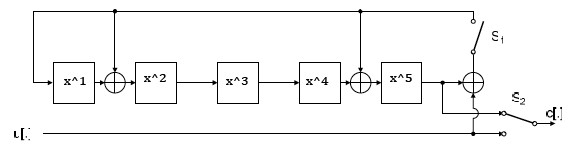
\includegraphics[width=11cm]{./bilder/shift_reg.png}
$\to$ \textbf{Polynom}: $g(x)=1+x^1+x^4+x^5$\\

\begin{list}{$\bullet$}{\setlength{\itemsep}{0cm} \setlength{\parsep}{0cm} \setlength{\topsep}{0.1cm}} 
\item Every cyclic shift of a code word is an other code word.
\item Two code words added give a new code word (so, 00..00 and 11..11 is often also a code word)
\item Generator Matrix $G$ are the linearly independent rows of the code word table.
\item Using Polynomials to represent a binary vector. \\
	  $u=(u_0, u_1,..u_{n-1}) \leftrightarrow u(X)=u_0 \cdot X^0 + u_1 \cdot X^1 + \ldots + u_{n-1} \cdot X^{n-1}$
\item Each code word $u$ corresponds to a polynomial $u(X)$ of degree $n-1$
\item In a $(n,k)$ cyclic code, there exists only one generator polynomial $g$ of degree $n-k$ with $g_0=1$
\end{list}

\subsubsection{Systematic Cyclic Codes (7,3)=(n,k)}
The code word $u$ must exhibit two properties:

\begin{list}{$\bullet$}{\setlength{\itemsep}{0cm} \setlength{\parsep}{0cm} \setlength{\topsep}{0.1cm}} 
  \item	It must be systematic: $u=(p_0,\ldots, p_{n-k-1}, m_0,\ldots,m_{k-1})$
  \item It must be a code word: $p(X)=X^{n-k}\cdot m(X) \mod g(X)$ \\
  \item $g(X)$ has the degree $n-k$ and must represent a valid code word
  \item The degree of $p(X)$ is always less than $n-k$
  \item $c=[p,m]$ (codeword)
  \item $s(X)=r(X)\mod g(X)$ (syndrom)
  \item $h(x)=X^n+1 : g(X)$ (check polynom)\\
        $H=\begin{bmatrix} 	
        			0	& \ldots	& \ldots	& 0 	& h_0		&	\ldots	&	h_m \\
        			0	& \ldots	& 0			& h_0	& \ldots	&	h_m		&	0	\\
        			\ldots &		&			&		&			&			&	\ldots \\
        			h_0	&	\ldots	& h_m		& 0		&	\ldots	&	\ldots	& 	0 \\
        \end{bmatrix}$  \\   
\end{list}
Achtung: in den Aufgaben ist LSB und MSB nicht wie gewohnt!\\

\subsubsection{Hamming Code}
$\alpha \to$ roots of the primitive polynomial.\\
\begin{list}{$\bullet$}{\setlength{\itemsep}{0cm} \setlength{\parsep}{0cm} \setlength{\topsep}{0.1cm}} 
  \item choose $m \geq 3$ (number of parity check equations)
  \item Length of code word $n=2^m-1$
  \item Length of message block $k=n-m$
  \item The Columns of the parity check matrix contain all integers between $1$ and $2^m-1$ as binary numbers. \\
		$H=[\ldots] $
  \item Every single bit error pattern yields a distinct syndrom vector
  \item checksum condition $\displaystyle\sum_{j=0}^{n-1}u_j \cdot \alpha^j = 0$
  \item where is the error:\\
  		$\displaystyle\sum_{j=0}^{n-1}r_j \cdot \alpha^j = \underbrace{\displaystyle\sum_{j=0}^{n-1}u_j \cdot \alpha^j}_{=0} + \underbrace{\displaystyle\sum_{j=0}^{n-1}e_j \cdot \alpha^j}_{=e_p \cdot \alpha^p}= \underbrace{\alpha^p}_{\text{error position}}$
  \item Parity check matrix: $H=[\alpha^0, \alpha^1, \ldots , \alpha^{n-1}]$

\end{list}

\subsubsection{BCH-Codes - Bose-Chaudhuri-Hocquenghem-Codes}
\begin{liste}
  \item choose a field $GF(2^m)$ for some positive integer m
  \item Let $\alpha$ be a primitive element of this field (root)
  \item A code word consists of $n=2^m-1$ binary digits. $u=(u_0, \ldots, u_{n-1})$
  \item Check sums $\displaystyle\sum_{i=0}^{n-1} u_i \cdot \alpha^{i \cdot q} = 0, \quad q=1,2,\ldots,r$
  \item This code can correct $t$ errors if $r \geq 2\cdot t-1$
  \item This code has $2^{n-rm}$ codewords
  \item even q are useless $\to \alpha=\alpha^2$ at $GF(2)$ $\to$ just evaluate the odd\\
     			$H=\begin{bmatrix} 	1 & \alpha   & \alpha^2     	& \ldots	& \alpha^{n-1} \\    		
   						   		1 & \alpha^3 & (\alpha^3)^2	& \ldots	& (\alpha^3)^{n-1}  \\    
   						   		1 & \alpha^5 & (\alpha^5)^2	& \ldots	& (\alpha^5)^{n-1}  \\   
   						   		\vdots	&	 &					&			& \vdots \\   						 
   						   		1 & \alpha^r & (\alpha^r)^2	& \ldots	& (\alpha^r)^{n-1}  \\   		
   			\end{bmatrix}$\\
\end{liste}

\subsection{RS Codes - Reed Solomon}
The code symbols $u_i$ are not binary digits but elements of $GF(q)$. However, if $q=2^m$, then every code symbol
can be represented by a binary vector of length m.\\


To build a systematic code with $k$-data symbols $(\bm m(X))$, $2t$ parity symbols and totally $k+2t=n$ symbols:
\begin{liste}
\item A primitive element $\alpha$ of $GF(2^m)$ has to be chosen. 
$\alpha$ is an element of order $2^m-1$: $\alpha^j\neq 1 \forall j\in [1,2^m-2]$; $\alpha^{2^m-1}=1$
\item The generator polynomial $\bm g(X)$ is:  $\bm g(X)=(X - \alpha^1) (X – \alpha^2)\ldots (X – \alpha^{2t})$
\item Calculate the parity symbols: $\bm p(X)=X^{n-k}\cdot \bm m(X) \mod \bm g(X)$
\item Sum up both together: $\bm u(X)=\bm p(X) +X^{n-k}\cdot \bm m(X) $
\item If the code word $\bm u(X) = u_0 + u_1 X+u_2 X^2\ldots+u_{n-1}X^{n-1} = ( u_0,  u_1, \ldots,  u_{n-1})$ is transformed into ``frequency space'', 
$U_k = \sum\limits_{i=0}^{n-1} u_i\cdot \alpha^{-i\cdot k}=\bm u(\alpha^{-k})$.
\item there have to be $2t$ zeros at the end of $\bm U=(U_0,U_1,\ldots,U_{k-1},0,\ldots,0)$
\end{liste}
e.g. (7,3)R-S code $(n=7, k=3 \Rightarrow 2t=4 \Rightarrow 2$ bit error correction$)$:
\begin{liste}
\item input: $\underbrace{010}_{\equiv a^1} \underbrace{110}_{\equiv a^3} \underbrace{111}_{\equiv a^5}$
\item input polynomial: $\bm m(X)=\alpha^1 + \alpha^3 X + \alpha^5 X^2$ 
\item The upshifted polynomial: $\bm m(X) X^{n-k}=\alpha^1 X^4 + \alpha^3 X^5 + \alpha^5 X^6$
\item calculate the parity polynomial: $\bm p(X)=\bm m(X) X^{n-k} \mod \bm g(X)\\
= \alpha^1 X^4 + \alpha^3 X^5 + \alpha^5 X^6 \mod \alpha^3 + \alpha^1 X + \alpha^0 X^2+\alpha^3 X^3+ X^4=\alpha^0+\alpha^2 X+\alpha^4 X^2 + \alpha^6 X^3$
\item $\bm u(X)=\alpha^0 + \alpha^2 X + \alpha^4 X^2 + \alpha^6 X^3+ \alpha^1 X^4 + \alpha^3 X^5 + \alpha^5 X^6$
\end{liste}
A correct code word is always a multiply of $\bm g(X)$ and has $2t$ zeros in the ``frequency space''. If not, this bit's represent the error pattern. 
To recalculate the \em error pattern \em the ``inverse DFT- inverse frequency transformation'' 
$e_i(X)=\frac{1}{n}\sum\limits_{k=1}^n E_k(X) \alpha^{i \cdot k}=\bm E(\alpha^i)$ has to used of the  error pattern $\bm E= \bm R - \bm U$.\\
An less power intensive variant is the \em Berlekamp-Massey Algorithm \em. It finds the shortest linear feedback shift register which generate the 
whole error pattern out of the last $2t$ frequency symbols $R_{n-2t},\ldots,R_{n-1}$ (If there are less then t errors.).

\begin{minipage}{9cm}
\textbf{DFT-Matrix Representation}
$V=v \cdot A$\\
 $A=\begin{bmatrix} 	
    	\alpha^{-0\cdot 0}		& \alpha^{-0\cdot 1}		& 	\ldots	&\alpha^{-0\cdot (n-1)}	\\
    	\alpha^{-1\cdot 0}		& \alpha^{-1\cdot 1}		& 	\ldots	&\alpha^{-1\cdot (n-1)}	\\
    	\alpha^{-2\cdot 0}		& \alpha^{-2\cdot 1}		&	\ldots	&\alpha^{-2\cdot (n-1)}	\\
    	\vdots					&							&			& \vdots				\\
    	\alpha^{-(n-1)\cdot 0}	& \alpha^{-(n-1)\cdot 1}	&  	\ldots	&\alpha^{-(n-1)\cdot (n-1)}	\\
    \end{bmatrix}$  \\    
\end{minipage}
\begin{minipage}{9cm}
\textbf{IDFT-Matrix Representation}
$v=V \cdot A^{-1}$\\
 $A^{-1}=\frac{1}{n}\cdot \begin{bmatrix} 	
    	\alpha^{0\cdot 0}		& \alpha^{0\cdot 1}		& 	\ldots	&\alpha^{0\cdot (n-1)}	\\
    	\alpha^{1\cdot 0}		& \alpha^{1\cdot 1}		& 	\ldots	&\alpha^{1\cdot (n-1)}	\\
    	\vdots					&						&			& \vdots			\\
    	\alpha^{(n-1)\cdot 0}	& \alpha^{(n-1)\cdot 1}	&	\ldots	&\alpha^{(n-1)\cdot (n-1)}	\\
    \end{bmatrix}$  \\    
\end{minipage}
 
\section{Convolutional Codes}
\subsection{TCM - Trellis Coded Modulation}
\subsubsection{Convolutional Coding - Faltungs Code}
Ein Faltungs Code besitzt zur Logikschaltung zus\"atzlich noch Memory, so dass
nicht nur der aktuelle Eingang sondern auch noch $n$-vorherige Eing\"ange zum
Ausgang verrechnet werden. Es gibt m unterschiedliche Ausg\"ange. 
Je nach Vorgeschichte, k\"onnen nur noch ganz bestimmte Kombinationen auftreten,
was dann die Decodierung besser macht.\\
\begin{minipage}{9cm}
	Beispiel mit k=1; n=2; m=2 $\to$ 1/2 codierung\\
	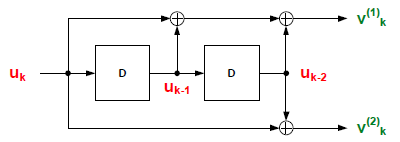
\includegraphics[width=9cm]{./bilder/covolutionSchemata.png}
\end{minipage}
\hspace{5mm}
\begin{minipage}{8cm}
\vspace{4mm}
	mit dazugeh\"origem Encoder State Diagram\\
\hspace{5mm}
	\includegraphics[width=6cm]{./bilder/covolutionStateDiagram.png}
\end{minipage}

\subsubsection{Decodierung}
Eine gute Variante die FaltungsCodes zu dekodieren ist dies mit einem Trellis
Diagram zu machen: \\
\begin{minipage}{10cm}
	\begin{liste}
		\item Zuerst Punkte entsprechend der m\"oglichen Speicherinhalte einzeichnen.
		\item M\"ogliche Verbindungen einzeichnen.
		\item Sollwerte einzeichnen (z.B. 0/00).
		\item Fehler zu den einzelnen Punkten eintragen (ev. die Euklidische Distanz).
		\item Wenn zwei Wege zu einem Punkt kommen, den h\"oherwertigen Weg streichen.
		\item Am Schluss den Weg nehmen der den kleinsten Fehler ergibt.
	\end{liste}
\end{minipage}
\begin{minipage}{9cm}
	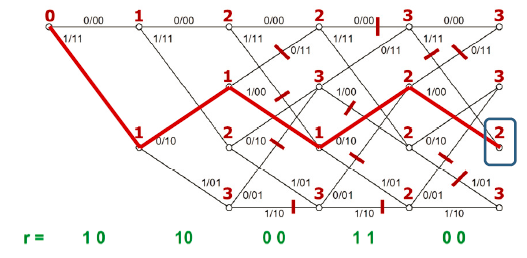
\includegraphics[width=9cm]{./bilder/Trelli.png}
\end{minipage}

\subsubsection{Euklidische Distanz}
\begin{minipage}{13cm}
	Die \textbf{euklidische Distanz} ist der Abstand zwischen zwei
	unterschiedlichen Modulationspositionen.\\
	Die \textbf{freie euklidische Distanz} ist der minimale Abstand zwischen zwei
	unterschiedlichen Modulationspositionen in der ganzen Modulation.\\
	$d^2_{free}=\min \limits_{a_k \neq a_{k}^{'}} \sum \limits_k
	d^2(a_k,a_{k}^{'})$\\
	zB.	$d^2_{min}=1 + 1 -2\cos (\alpha)= 2-\sqrt{2} = 0.586$\\
	Der \textbf{Coding Gain} ist um welchen Faktor der SNR schlechter sein darf.\\
	$G = \frac{d^2_{free,coded}}{d^2_{min, uncoded}}$
\end{minipage}
\begin{minipage}{6cm}
	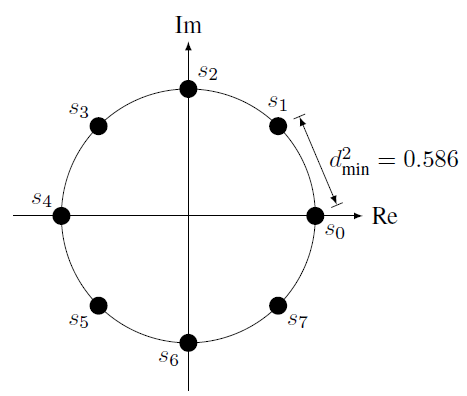
\includegraphics[width=6cm]{./bilder/EuklidischeDistanz.png}
\end{minipage} 

%\input{Content/PadePronyShank/PadePronyShank}
\newpage



\end{document}
